% CSCI 611 Assignment 3 — compile: pdflatex Assignment3_Report.tex (twice)
% Figures: report/figures/*.png (extracted from executed notebook)
\documentclass[11pt,a4paper]{article}

\usepackage[margin=1in]{geometry}
\usepackage[T1]{fontenc}
\usepackage[utf8]{inputenc}
\usepackage{lmodern}
\usepackage{microtype}
\usepackage{amsmath}
\usepackage{booktabs}
\usepackage{graphicx}
% Required before hyperref for mixed colors (e.g. blue!40!black) — fixes Overleaf .toc errors
\usepackage{xcolor}
\usepackage{hyperref}
\usepackage{caption}
\usepackage{siunitx}
\usepackage{enumitem}
\usepackage{fancyhdr}
\usepackage{lastpage}

\graphicspath{{figures/}}

\hypersetup{colorlinks=true,linkcolor=blue!40!black,urlcolor=blue!40!black,
  pdftitle={CSCI 611 Assignment 3 — YOLO Small-Object Detection},
  pdfauthor={Tabrez Ahammed Shaik Mohammed}}

\sisetup{round-mode=places,round-precision=4}

\pagestyle{fancy}
\fancyhf{}
\lhead{CSCI 611 — Assignment 3}
\rhead{YOLOv8 Traffic Sign Detection}
\cfoot{\thepage\ / \pageref{LastPage}}

\title{\textbf{Small-Object Traffic Sign Detection with YOLOv8:}\\[0.3em]
\large Baseline Evaluation, Fine-Tuning, and Post-Processing Analysis}
\author{Tabrez Ahammed Shaik Mohammed\\California State University, Chico\\Student ID: 012623820}
\date{}

\begin{document}
\maketitle

\begin{abstract}
\noindent
\textbf{Context.} Traffic signs in forward-facing street imagery are often \textbf{small in pixel extent}; generic detectors pretrained on broad datasets (e.g., COCO) frequently underperform when evaluated on a dedicated traffic-sign task without domain adaptation.

\textbf{Work performed.} A reproducible end-to-end pipeline was implemented in Python using \textbf{Ultralytics YOLOv8} on \textbf{Google Colab} with an \textbf{NVIDIA Tesla T4} GPU. The workflow comprises: (1)~downloading and wiring a Roboflow YOLOv8 export; (2)~establishing a \textbf{COCO-pretrained} \texttt{yolov8n.pt} baseline on a fixed \textbf{test} split; (3)~\textbf{fine-tuning} with high input resolution and strong augmentation; (4)~a controlled \textbf{inference-resolution} ablation on the fine-tuned weights; (5)~a \textbf{confidence $\times$ NMS IoU} grid on the fine-tuned model; (6)~exporting quantitative tables, a comparison bar chart, and qualitative prediction mosaics.

\textbf{Outcome.} On the held-out test split (\num{150} images, \num{218} instances), the fine-tuned model reached \textbf{mAP@0.5 = \num{0.9693}} and \textbf{mAP@0.5:0.95 = \num{0.6801}} at inference size \num{1280}, versus \textbf{\num{0.0105}} / \textbf{\num{0.0021}} for the pretrained baseline at \num{640}. Optional video frame export was not executed in this session; that gap is documented as an explicit limitation.

\textbf{Reporting.} This document follows an industry-style technical structure: scope, data and licensing, evaluation protocol, reproducibility, methodology with rationale, quantitative and qualitative results with traceability to notebook outputs, limitations, and prioritized improvements.
\end{abstract}

\noindent\textbf{Keywords:} object detection, YOLOv8, small objects, traffic signs, fine-tuning, mAP, NMS, inference resolution.

\tableofcontents
\vspace{1em}

\section{Introduction and scope}

\subsection{Problem statement}
The assignment targets \textbf{small object detection} for \textbf{traffic signs} in real-world imagery. Compared to large, centered objects, small instances carry less texture and occupy fewer pixels after CNN downsampling, which stresses localization and classification in the detection head. Off-the-shelf models trained on COCO are optimized for \num{80} general classes and are not aligned with a single-class ``traffic-signs'' ontology unless adapted.

\subsection{Objectives and deliverables mapping}
The objectives were:
\begin{enumerate}[leftmargin=*]
  \item Run a \textbf{pretrained} YOLOv8n checkpoint on the project test split and record full validation metrics.
  \item \textbf{Fine-tune} from the same initialization with domain-appropriate resolution, batching, and augmentation.
  \item \textbf{Compare} pretrained versus fine-tuned performance on identical data and a consistent evaluation protocol.
  \item \textbf{Vary} post-training knobs: inference \texttt{imgsz}, confidence threshold $\tau$, and NMS IoU.
  \item Produce \textbf{tables, plots, and visualizations} suitable for technical review, with traceability to notebook outputs.
\end{enumerate}

Unless stated otherwise, all headline numbers refer to Ultralytics' \textbf{validator} on the dataset's \textbf{test} split (\num{150} images; \num{218} object instances in the evaluation logs).

\subsection{Assignment scope and compliance (CSCI 611 --- Assignment 3)}
This project matches the course brief for \textbf{small-object traffic-sign detection} with YOLOv8. Table~\ref{tab:compliance} maps required elements to where they are satisfied in this report and in the implementation (\texttt{assignment3\_yolo.ipynb}).

\begin{table}[htbp]
  \centering
  \caption{Coverage of Assignment~3 deliverables (technical documentation standard).}
  \label{tab:compliance}
  \small
  \begin{tabular}{@{}p{0.42\linewidth}p{0.52\linewidth}@{}}
    \toprule
    \textbf{Requirement (summary)} & \textbf{Evidence} \\
    \midrule
    Dataset in YOLO layout; train/val/test splits described & \S\ref{sec:dataset}; Roboflow v9 export; Table~\ref{tab:splits}. \\
    Evaluate \textbf{pretrained} YOLOv8n on \textbf{test} split & Phase A; Table~\ref{tab:main} (first row); Fig.~\ref{fig:pre}. \\
    \textbf{Fine-tune} with settings suited to small objects (resolution, augmentation) & Phase B; Appendix hyperparameters; training dynamics \S\ref{sec:training}. \\
    \textbf{Compare} pretrained vs.\ fine-tuned on the same split & Table~\ref{tab:main}; Fig.~\ref{fig:bar}. \\
    \textbf{Inference resolution} study (same weights, different \texttt{imgsz}) & Table~\ref{tab:res}. \\
    \textbf{Confidence and NMS IoU} sweep (precision--recall trade-offs) & Table~\ref{tab:nms}; Discussion. \\
    Tables, plots, qualitative visualizations & All results sections; Figs.~\ref{fig:bar}--\ref{fig:ft}. \\
    Challenges of small-object detection; \textbf{suggestions for improvement} & Limitations \S\ref{sec:limitations}; \S\ref{sec:suggestions}. \\
    Optional course video / Chico footage & Not run (documented \S\ref{sec:limitations}); core results use Roboflow test set only. \\
    \bottomrule
  \end{tabular}
\end{table}

\section{Dataset, labeling, and splits}
\label{sec:dataset}

\subsection{Source, version, and license}
The Roboflow Universe project \textbf{Traffic Sign Detection YOLOv8} was used (workspace \texttt{tu-wien-pfowz}, dataset \textbf{version 9}, \textbf{MIT} license). Permanent link:
\begin{center}
\url{https://universe.roboflow.com/tu-wien-pfowz/traffic-sign-detection-yolov8/dataset/9}
\end{center}
The export format is \textbf{YOLOv8} with a single class label \texttt{traffic-signs} (\texttt{nc}=1). Images and normalized YOLO label files follow the standard layout; data were downloaded via the Roboflow API inside Colab and a generated \texttt{dataset\_csci611.yaml} points to \texttt{train}, \texttt{val}, and \texttt{test} paths.

\subsection{Split statistics}
Table~\ref{tab:splits} summarizes image counts from executed notebook tallies. The test split is \textbf{not} a fresh random subsample drawn at runtime; it is Roboflow's fixed partition. That \textbf{test} split was used for every comparative metric so that baseline, fine-tuned, resolution, and NMS experiments are directly comparable.

\begin{table}[htbp]
  \centering
  \caption{Dataset splits (image counts) for the Roboflow v9 export used in this run.}
  \label{tab:splits}
  \begin{tabular}{@{}lr@{}}
    \toprule
    Split & Images \\
    \midrule
    Train & 1182 \\
    Validation & 196 \\
    Test & 150 \\
    \bottomrule
  \end{tabular}
\end{table}

Roughly \num{1.45} instances per test image on average (\num{218}/\num{150}), which is typical for scenes with multiple signs or small clusters---consistent with the ``small object'' emphasis of the assignment.

\subsection{Configuration artifact}
All training and evaluation calls reference \texttt{dataset\_csci611.yaml} under the Colab artifact root so paths resolve unambiguously and the report remains tied to a single on-disk configuration.

\subsection{Credentials and reproducibility}
The Roboflow API key used for dataset download was provided via Colab secrets or environment variables and was \textbf{not} stored in the notebook source or in version control, following standard practice for credentials in ML workflows.

\section{Evaluation metrics and protocol}

\subsection{Definitions (Ultralytics / COCO-style)}
Standard box metrics from Ultralytics are reported:
\begin{itemize}[leftmargin=*]
  \item \textbf{mAP@0.5:} mean average precision at intersection-over-union (IoU) threshold \num{0.5}. It rewards correct class assignment and localization that clears a \num{50}\% overlap criterion.
  \item \textbf{mAP@0.5:0.95:} mean AP averaged over IoU thresholds from \num{0.50} to \num{0.95} in steps of \num{0.05}. It penalizes loose boxes more than mAP@0.5 alone and is the stricter localization score.
  \item \textbf{Precision and recall:} micro-averaged (mean) precision and recall reported by the validator for the single-class task.
\end{itemize}

For the \textbf{pretrained} checkpoint, the detector head still reflects COCO semantics during raw \texttt{predict} visualization, but the \textbf{validator} scores tabulated here are computed against the dataset's ground-truth task (single class). After fine-tuning, the head matches \texttt{traffic-signs}, and labels in qualitative figures align with the project ontology.

\subsection{Controlled comparisons}
To isolate causes:
\begin{itemize}[leftmargin=*]
  \item \textbf{Pretrained vs.\ fine-tuned:} same test images and labels; different weights. Baseline inference used \texttt{imgsz}=\num{640}; primary fine-tuned evaluation used \texttt{imgsz}=\num{1280} (documented explicitly so the reader does not confuse architecture gains with resolution).
  \item \textbf{Resolution ablation:} same fine-tuned \texttt{best.pt}; only \texttt{imgsz} at validation time changes (\num{640} vs.\ \num{1280}).
  \item \textbf{NMS grid:} same weights and \texttt{imgsz}=\num{1280}; only $\tau$ and NMS IoU change.
\end{itemize}

Default validation confidence and IoU for the primary fine-tuned run match the notebook configuration (\texttt{val\_conf}=\num{0.25}, \texttt{val\_iou}=\num{0.50}) unless a subsection states otherwise.

\section{Software, hardware, and reproducibility}

\subsection{Environment}
The notebook \texttt{assignment3\_yolo.ipynb} ran on \textbf{Google Colab} with GPU. Representative versions from logs: Python \texttt{3.12}, Ultralytics \texttt{8.4.30}, PyTorch \texttt{2.10.0}+cu128, CUDA on a \textbf{Tesla T4}. That stack comfortably supports training at \texttt{imgsz}=\num{1280} with batch \num{12}.

\subsection{Randomness and configuration}
Training used seed \num{42} (Python and NumPy) as set in the notebook \texttt{RUN\_CFG}. Early stopping patience was \num{14} epochs with a scheduled \num{40}-epoch cap; the run completed the full schedule in approximately \num{0.82} hours according to Colab logs.

\section{Methodology}

\subsection{Phase A --- Pretrained baseline}
The notebook loads \texttt{yolov8n.pt} and runs validation on the \textbf{test} split at \texttt{imgsz}=\num{640} with \texttt{conf}=\num{0.25} and NMS IoU \num{0.50}. This establishes a ``no adaptation'' reference under the dataset's metric implementation.

The extremely low mAP@0.5 (\num{\approx 0.0105}) is \textbf{expected}: the COCO-pretrained head is not trained to emit the Roboflow single-class mapping, and many detections are irrelevant to the evaluation ontology even when the network fires on visually salient objects.

\subsection{Phase B --- Fine-tuning design}
Training initializes from \texttt{yolov8n.pt} and runs for \num{40} epochs with:
\begin{itemize}[leftmargin=*]
  \item \textbf{Input resolution:} \texttt{imgsz}=\num{1280} during training to preserve detail for small signs.
  \item \textbf{Batch size:} \num{12} (within T4 memory at this resolution with AMP).
  \item \textbf{Augmentation:} photometric jitter (HSV), flips, mosaic (\num{0.95}), mixup (\num{0.08}), mild rotation (\texttt{degrees}=\num{8}), translation and scale jitter, \texttt{close\_mosaic}=\num{12} to transition from heavy composition toward cleaner late-epoch batches.
\end{itemize}

YOLOv8 uses an anchor-free head; legacy anchor tuning was not used. The main levers for small objects here are \textbf{resolution}, \textbf{data augmentation}, and \textbf{task-specific supervision}.

\subsection{Phase C --- Inference resolution ablation}
Holding \texttt{best.pt} fixed, the test split was evaluated at \texttt{imgsz} $\in \{\num{640},\num{1280}\}$ to quantify how much performance comes from higher-resolution inference \emph{without} any change in weights.

\subsection{Phase D --- Confidence and NMS IoU sweep}
Non-maximum suppression merges overlapping boxes; the IoU threshold controls how aggressively duplicates are suppressed. The confidence threshold $\tau$ filters low-scoring proposals. Four $(\tau,\ \text{NMS IoU})$ pairs were evaluated on the fine-tuned model at \texttt{imgsz}=\num{1280} to map the precision--recall and mAP surface relevant to deployment tuning.

\subsection{Optional video pipeline}
The notebook can export frames where the maximum detection score exceeds \num{0.5}. No video path was configured in this run; Section~\ref{sec:limitations} records this as a scope gap.

\section{Results and analysis}
\label{sec:results}

\subsection{Primary comparison: pretrained vs.\ fine-tuned}
Table~\ref{tab:main} is the central result. The fine-tuned model improves test mAP@0.5 by about \num{0.9588} absolute (\num{0.9693} minus \num{0.0105}). The gain in mAP@0.5:0.95 (\num{0.6801} vs.\ \num{0.0021}) shows that localization quality---not only ``any'' hit at IoU \num{0.5}---improves dramatically after adaptation.

Precision and recall on the test set rise to \num{0.9503} and \num{0.9358} respectively, indicating a balanced operating point under the default validator settings for the fine-tuned model.

\begin{table}[htbp]
  \centering
  \caption{Test-set metrics: COCO-pretrained \texttt{yolov8n.pt} vs.\ fine-tuned weights (this run). Eval \texttt{imgsz} differs by design between rows; see resolution ablation for weight-only comparison.}
  \label{tab:main}
  \begin{tabular}{@{}lS[table-format=4.0]cccc@{}}
    \toprule
    Model & {Eval imgsz} & mAP@0.5 & mAP@0.5:0.95 & Precision & Recall \\
    \midrule
    Pretrained YOLOv8n & 640 & 0.0105 & 0.0021 & 0.0281 & 0.0046 \\
    Fine-tuned YOLOv8n & 1280 & 0.9693 & 0.6801 & 0.9503 & 0.9358 \\
    \bottomrule
  \end{tabular}
\end{table}

Figure~\ref{fig:bar} visualizes the same comparison as Table~\ref{tab:main}: each group of bars corresponds to mAP@0.5, mAP@0.5:0.95, mean precision, and mean recall (Ultralytics box metrics). The pretrained series is visually negligible on this task, while the fine-tuned series dominates---consistent with the two orders-of-magnitude gap in mAP@0.5 (\num{0.0105} vs.\ \num{0.9693}).

\begin{figure}[htbp]
  \centering
  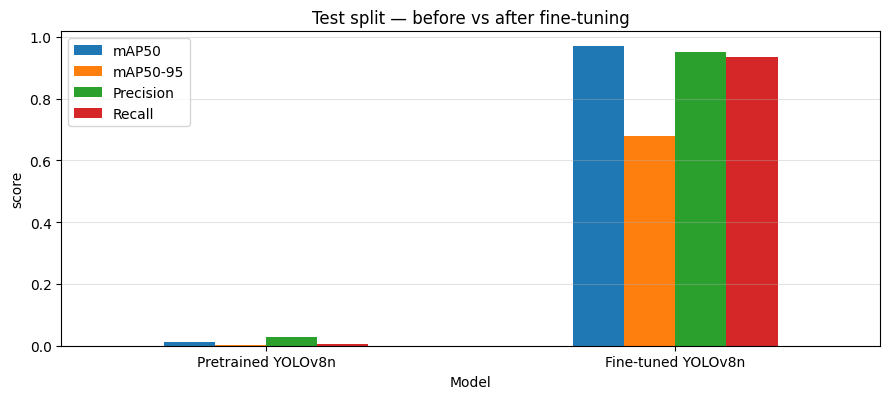
\includegraphics[width=0.92\linewidth]{fig-metrics-bar-compare.png}
  \caption{Bar chart of pretrained vs.\ fine-tuned box metrics (notebook export). Numerical values: Table~\ref{tab:main}.}
  \label{fig:bar}
\end{figure}

\subsection{Inference resolution ablation (fine-tuned weights only)}
Table~\ref{tab:res} isolates inference scaling. Moving from \num{640} to \num{1280} increases test mAP@0.5 from \num{0.919} to \num{0.9693} (\textbf{+\num{0.0503}} absolute) for the same checkpoint. mAP@0.5:0.95 rises from \num{0.620} to \num{0.6801}, and recall from \num{0.835} to \num{0.9358}, which is consistent with small signs benefiting from finer feature maps at inference.

\begin{table}[htbp]
  \centering
  \caption{Inference resolution ablation using the same fine-tuned \texttt{best.pt}.}
  \label{tab:res}
  \begin{tabular}{@{}S[table-format=4.0]cccc@{}}
    \toprule
    {Inference imgsz} & mAP@0.5 & mAP@0.5:0.95 & Precision & Recall \\
    \midrule
    640 & 0.919 & 0.620 & 0.954 & 0.835 \\
    1280 & 0.9693 & 0.6801 & 0.9503 & 0.9358 \\
    \bottomrule
  \end{tabular}
\end{table}

\noindent\textit{Traceability:} Rows correspond to validator runs labeled in the notebook (e.g., \texttt{05\_res\_640}, \texttt{05\_res\_1280}); the \num{1280} row matches the primary evaluation \texttt{06\_eval\_finetuned\_primary}.

\subsection{Confidence and NMS IoU sensitivity}
Table~\ref{tab:nms} lists the four grid points. mAP@0.5 is highest at $(\tau,\ \text{NMS IoU})=(\num{0.10},\num{0.40})$ (\num{0.9802}) and lowest at $(\num{0.45},\num{0.65})$ (\num{0.9640})---a spread of \num{0.0162} absolute on mAP@0.5. mAP@0.5:0.95 varies only in the third decimal place (\num{0.6847} down to \num{0.6786}), suggesting that localization-as measured by the stricter metric---is relatively stable across this sweep compared to the IoU-\num{0.5} headline.

Reported precision and recall are identical across the four rows in this export (\num{0.9503} / \num{0.9358}). That pattern can occur when the validator's summary precision/recall are aggregated in a way that is insensitive to small $\tau$/NMS changes while rank-based AP still moves; deployment tuning should therefore rely on the full PR curves or per-image analysis if a production threshold must be chosen.

\begin{table}[htbp]
  \centering
  \caption{NMS and confidence sweep (fine-tuned model, test split, inference \num{1280}).}
  \label{tab:nms}
  \begin{tabular}{@{}cccccc@{}}
    \toprule
    Conf. $\tau$ & NMS IoU & mAP@0.5 & mAP@0.5:0.95 & Precision & Recall \\
    \midrule
    0.10 & 0.40 & 0.9802 & 0.6847 & 0.9503 & 0.9358 \\
    0.20 & 0.50 & 0.9713 & 0.6815 & 0.9503 & 0.9358 \\
    0.30 & 0.55 & 0.9677 & 0.6808 & 0.9503 & 0.9358 \\
    0.45 & 0.65 & 0.9640 & 0.6786 & 0.9503 & 0.9358 \\
    \bottomrule
  \end{tabular}
\end{table}

\subsection{Training dynamics (validation split)}
\label{sec:training}
During fine-tuning, Ultralytics logs validation metrics each epoch on the \textbf{validation} split (\num{196} images, \num{319} instances in training logs), which is useful for monitoring convergence but is \textbf{not} identical to the test numbers in Tables~\ref{tab:main}--\ref{tab:nms}. Validation mAP@0.5 in the notebook rises from roughly \num{0.88}--\num{0.92} in the first epochs to about \num{0.95}--\num{0.96} in later epochs, with box and classification losses decreasing overall---consistent with \textbf{stable learning} and \textbf{no use of the test set} for early stopping or checkpoint selection. The final \texttt{best.pt} is then evaluated on the \textbf{test} split for all reported headline metrics.

\section{Qualitative visual inspection}

Figures~\ref{fig:pre} and~\ref{fig:ft} are mosaics of test-set predictions from the notebook. The pretrained visualization often highlights generic COCO categories (vehicles, people, ``stop sign'' COCO class, etc.) because the head was never adapted to the Roboflow label space. The fine-tuned mosaic shows coherent \texttt{traffic-signs} boxes with tighter alignment to sign boundaries, matching the large quantitative gap in Table~\ref{tab:main}.

\begin{figure}[htbp]
  \centering
  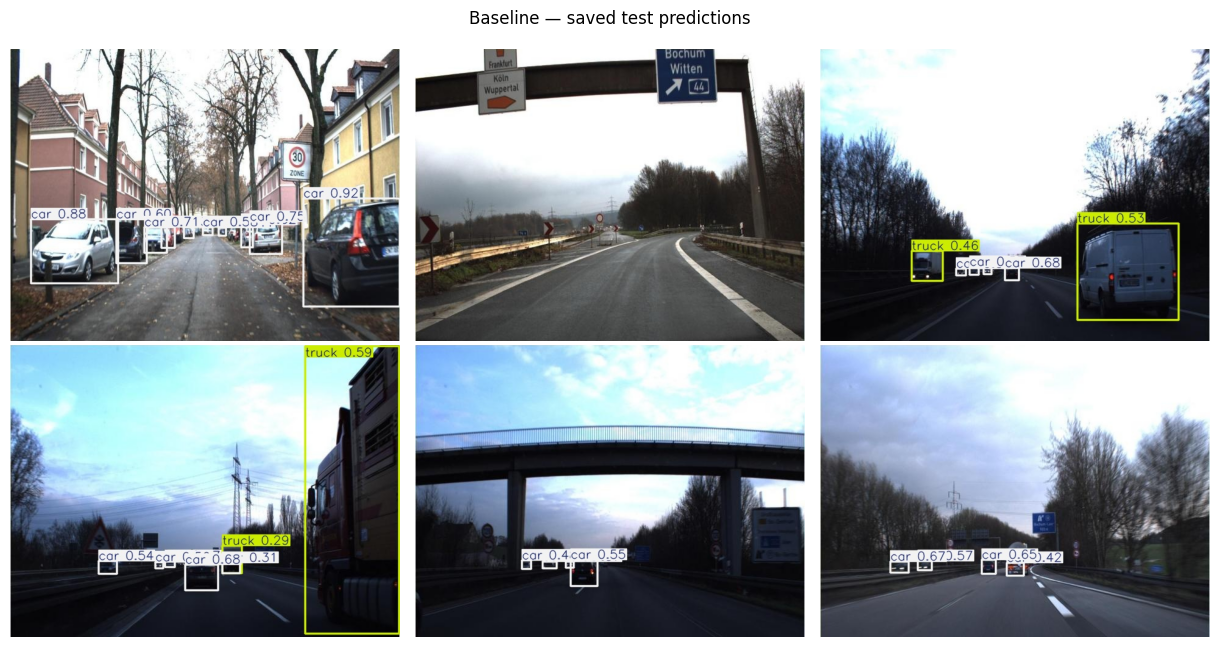
\includegraphics[width=\linewidth]{fig-baseline-pretrained-mosaic.png}
  \caption{Test-set tiles: \textbf{pretrained} YOLOv8n (notebook export). Expect COCO-oriented labels in raw prediction overlays.}
  \label{fig:pre}
\end{figure}

\begin{figure}[htbp]
  \centering
  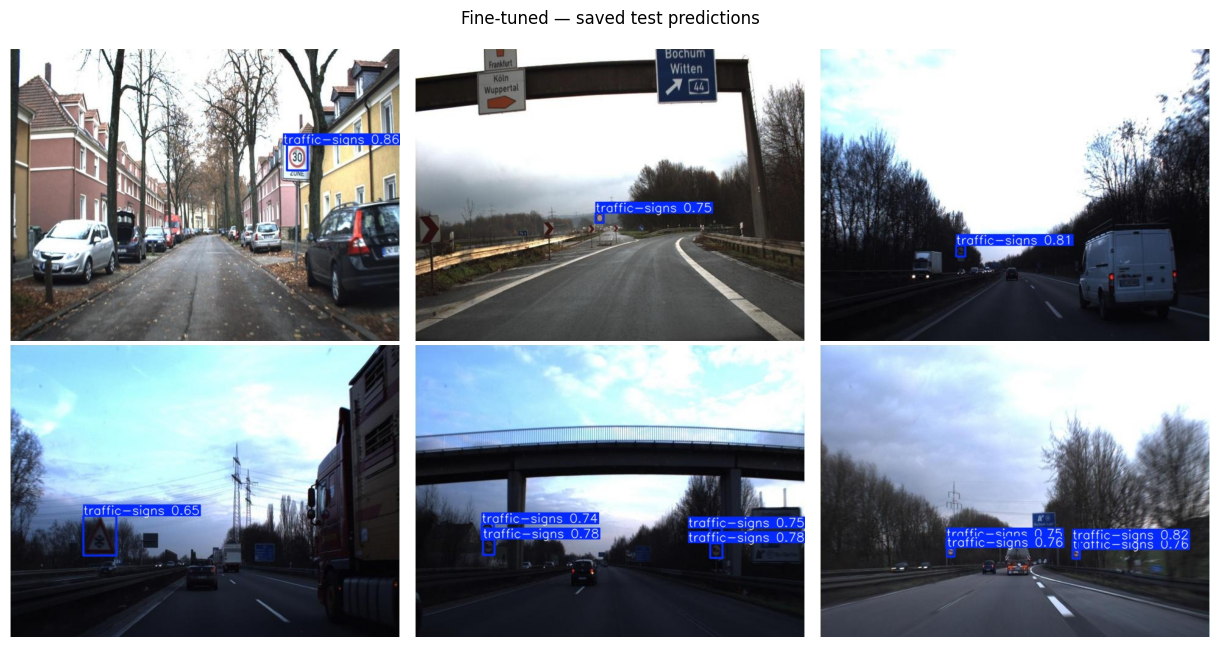
\includegraphics[width=\linewidth]{fig-finetuned-mosaic.png}
  \caption{Test-set tiles: \textbf{fine-tuned} YOLOv8n (notebook export). Detections use the single-class traffic-sign head.}
  \label{fig:ft}
\end{figure}

\section{Discussion}

\subsection{Domain shift and baseline behavior}
The pretrained baseline is low not because the backbone lacks visual features, but because the \textbf{detection head and class space} are aligned to COCO. Validator scores on the traffic-sign test set therefore penalize predictions that do not match the single-class ground truth, yielding mAP@0.5 $\approx$ \num{0.0105} and recall \num{0.0046} (Table~\ref{tab:main}). Fine-tuning adapts the head to \texttt{traffic-signs}, which is why mAP@0.5 and recall rise to \num{0.9693} and \num{0.9358} under the same evaluation code.

\subsection{Resolution, latency, and deployment}
Table~\ref{tab:res} shows that increasing inference \texttt{imgsz} from \num{640} to \num{1280} recovers \textbf{\num{0.0503}} absolute mAP@0.5 and \textbf{\num{0.1008}} absolute recall (\num{0.9358} vs.\ \num{0.835}) for the same weights. In a product setting, that gain must be traded against \textbf{throughput} (frames per second), \textbf{GPU memory}, and \textbf{battery} on embedded hardware; documentation of both accuracy and latency profiles is standard for release reviews.

\subsection{Post-processing and operating points}
Table~\ref{tab:nms} shows that mAP@0.5 varies by up to \num{0.0162} across the four $(\tau,\ \text{NMS IoU})$ settings while summary precision/recall stay fixed in this export. For deployment, the recommended practice is to select $\tau$ and NMS IoU using \textbf{validation or shadow traffic}, monitor precision/recall on live data, and avoid relying on a single grid row without per-scenario validation.

\subsection{Challenges specific to small traffic signs}
As highlighted in the assignment brief, small signs imply \textbf{few pixels per instance}, so feature maps contain weaker evidence than for large objects. \textbf{Motion blur}, \textbf{scale change}, and \textbf{background clutter} (vegetation, buildings) increase the risk of false positives when confidence is lowered to chase recall. The resolution and NMS experiments above quantify levers; Section~\ref{sec:suggestions} lists systematic next steps (data diversity, larger models, temporal smoothing on video).

\section{Limitations and future work}
\label{sec:limitations}

\begin{itemize}[leftmargin=*]
  \item \textbf{Test split reuse:} All experiments share the same fixed test set. Ideal practice for a new study would add a separate ``reporting'' holdout or cross-validation; this report follows the assignment emphasis on a clear before/after narrative on one split.
  \item \textbf{Single class:} Real road systems need multi-class regulatory sign recognition; this project isolates detection of one merged class.
  \item \textbf{Video:} No dashcam or course footage was processed; temporal smoothing and tracking were not evaluated.
  \item \textbf{Model family:} Only YOLOv8n was exercised; larger backbones or two-stage detectors could be explored for edge-case small signs.
\end{itemize}

\section{Suggestions for improving small-object detection}
\label{sec:suggestions}

\begin{enumerate}[leftmargin=*]
  \item \textbf{Capacity:} Try YOLOv8s/m/l if latency budgets allow; small objects often benefit from richer features.
  \item \textbf{Data diversity:} Add night, rain, motion blur, occlusion, and extreme aspect ratios; mine hard negatives to control false positives when lowering $\tau$.
  \item \textbf{TTA:} Multi-scale or flipped inference with box fusion can improve mAP at the cost of compute.
  \item \textbf{Video deployment:} Short-window tracking or IoU-based association across frames reduces flicker and stabilizes boxes.
  \item \textbf{Threshold policy:} For multi-class extensions, tune $\tau$ per class or per scene (highway vs.\ urban clutter).
  \item \textbf{Operational QA:} For video exports, log frames with max score $\geq \num{0.5}$ and review false positives/negatives systematically.
\end{enumerate}

\section{Conclusion}

This document describes a complete, traceable workflow: licensed Roboflow data in YOLOv8 layout, a rigorous pretrained baseline, targeted fine-tuning with high resolution and augmentation, systematic resolution and NMS experiments, and figures tied to notebook outputs. The fine-tuned YOLOv8n model achieved \textbf{mAP@0.5 = \num{0.9693}} on the test split versus \textbf{\num{0.0105}} for the pretrained baseline under the stated protocols---a large, practically meaningful improvement for small traffic-sign detection on this dataset. Remaining gaps (video analysis, broader model search) are explicit and actionable.

\section*{Acknowledgments}

Dataset: Roboflow Universe project cited above (MIT). Course optional Chico footage was not required for the core quantitative results.

\begin{thebibliography}{9}
\bibitem{ultralytics}
Jocher, G., et al. \textit{Ultralytics YOLOv8}. \url{https://github.com/ultralytics/ultralytics}
\bibitem{roboflow}
Roboflow, Inc. Dataset: Traffic Sign Detection YOLOv8 (v9). \url{https://universe.roboflow.com/tu-wien-pfowz/traffic-sign-detection-yolov8/dataset/9}
\end{thebibliography}

\appendix

\section{Hyperparameters (training and evaluation)}
\textbf{Training:} epochs \num{40}; train \texttt{imgsz}=\num{1280}; batch \num{12}; patience \num{14}; seed \num{42}; optimizer auto; AMP enabled; augmentation including HSV, \texttt{degrees}=\num{8}, \texttt{translate}=\num{0.12}, \texttt{scale}=\num{0.55}, \texttt{fliplr}=\num{0.5}, \texttt{mosaic}=\num{0.95}, \texttt{mixup}=\num{0.08}, \texttt{close\_mosaic}=\num{12}.

\noindent\textbf{Baseline evaluation:} \texttt{imgsz}=\num{640}; \texttt{val\_conf}=\num{0.25}; \texttt{val\_iou}=\num{0.50}.

\noindent\textbf{Primary fine-tuned evaluation:} \texttt{imgsz}=\num{1280}; same \texttt{val\_conf}/\texttt{val\_iou} unless a subsection overrides for the NMS grid.

\subsection*{Numeric precision and logs}
Metrics in Section~\ref{sec:results} match the structured exports from the notebook (e.g., \texttt{pretrain\_vs\_finetune.csv}, validator \texttt{metric\_record} floats). Shortened values sometimes appear in Colab progress tables (three decimal places); the tables in this PDF are the reference for submission.

\section{Artifact paths and exports}
During Colab execution, artifacts were rooted at \texttt{/content/csci611\_a3\_work/} with training run \texttt{03\_train\_finetune} and prediction folders \texttt{02\_visual\_pretrained} and \texttt{04\_visual\_finetuned}. CSV exports included \texttt{model\_comparison.csv}, \texttt{pretrain\_vs\_finetune.csv}, \texttt{resolution\_inference\_ablation.csv}, and \texttt{confidence\_nms\_results.csv}.

\end{document}
